\section{Introduction}
\begin{frame}{Introduction}
    % Slide 1: Introduction to HS
        \begin{columns}
        \column{0.65\textwidth}
            \begin{itemize}
                \item HS is an acknowledged phenomenon:
                \begin{itemize}
                    \item Social media platforms
                    \item Increasingly sheer volume of content
                    \item Change of policies
                \end{itemize}
                \item Targets:
                \begin{itemize}
                    \item LGTBQ+
                    \item Black community
                    \item \textbf{Women}
                    \item \textbf{Immigrants}
                \end{itemize} 
                \item Hate speech incites violence and intolerance
                \item Transformers for addressing HS
            \end{itemize}
        \column{0.35\textwidth}
                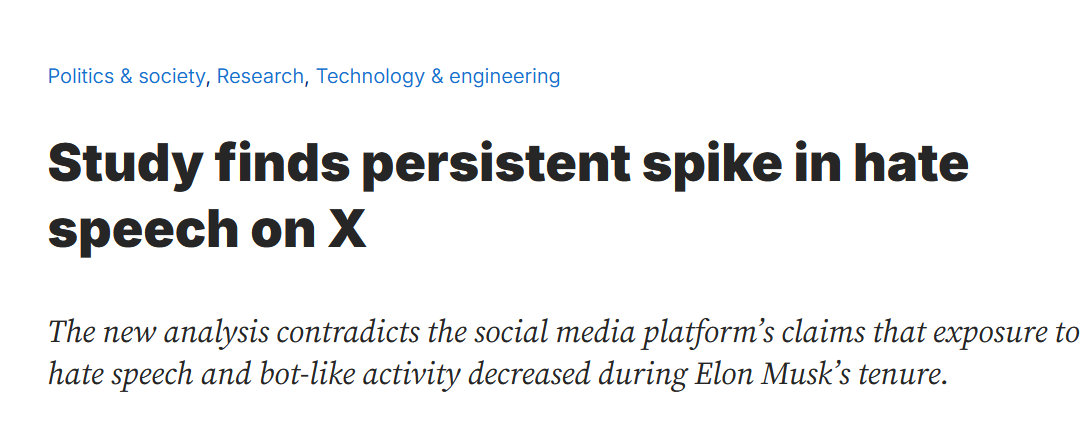
\includegraphics[width=\textwidth]{images/x_hate.PNG}
                \vfill
                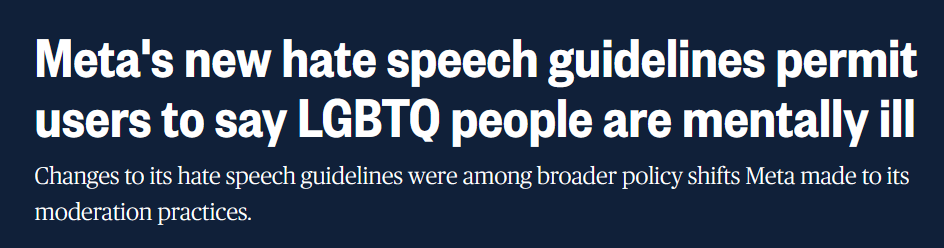
\includegraphics[width=\textwidth]{images/meta_new_policy.PNG}
                \vfill
                
\includegraphics[width=\textwidth]{images/homofobia.PNG}
        \end{columns}
        \footfullcite{oberaxe}
\end{frame}

\begin{frame}{Challenges of addressing HS}
    \begin{columns}
        \column{0.5\textwidth}
        \begin{itemize}
            \item Lack of a universal definition
        \item Intersection with various fields/areas
        \item Lack of resources outside of English
        \item Forms of expression:
            \begin{itemize}
        \item Aggressive: threats, violence
        \item Non-aggressive: humor, irony, \textbf{stereotypes}
            \end{itemize}
        \item Type of content:
            \begin{itemize}
            \item Text (mostly addressed)
            \item Multimodal (images, videos, \textbf{memes})
            \end{itemize}
        \item \textbf{Subjectivity}
        \end{itemize}
        \column{0.6\textwidth}
        \begin{quote}
            \textit{[...] the lack of definitions in scholarship translates to uncertain definitions
            in law and social science research, and even more uncertain application of
            principles in on-line spaces}
        \end{quote}
        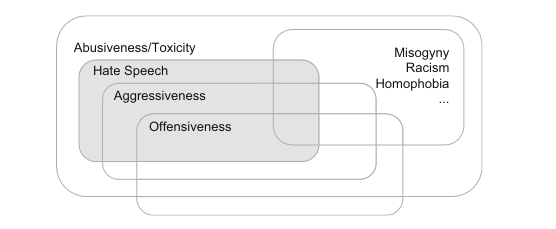
\includegraphics[width=\textwidth]{images/marco-hate.png}
\end{columns}
\footfullcite{sellars2016defining,Poletto2021}
\end{frame}

\begin{frame}{Deep learning and HS}

    \only<1->{\begin{alertblock}{DL limitations in HS}
        It is clear that automated methods, especially those based on DL, are necessary to address HS. However, the usage of black box methods involves ethical concerns.
    \end{alertblock}
    }
    \only<2->{
    \begin{block}{Addressing the limitations}
        What if we trained our models to see beyond black and white? What if we had more debiased datasets? What if we paid attention to all opinions?
    \end{block}
    }
\end{frame}

\begin{frame}{Research Questions}
    \begin{itemize}
        \item \textbf{RQ1}: How does the LeWiDi paradigm influence a classifier performance for detecting racial stereotypes in online comments and discussion forums?
        \item \textbf{RQ2}: How does the LeWiDi paradigm influence a classifier performance for detecting sexist stereotypes in memes?
        \item Shared tasks:
        \begin{itemize}
            \item \textbf{DETEST-Dis}: \textit{DETEction and classification of racial STereotypes in Spanish - Learning with Disagreement}
            \item \textbf{EXIST}: \textit{sEXism Identification in Social neTworks}
        \end{itemize} 
    \end{itemize}
\end{frame}